\documentclass[12pt]{article}
\usepackage[utf8]{inputenc}
\usepackage{amsmath}
\usepackage{systeme}
\usepackage{amsfonts}
\usepackage{graphicx}
\usepackage{enumitem}
\usepackage{hyperref}
\usepackage{xcolor}
\usepackage{kbordermatrix}
\usepackage{centernot}
\usepackage{xcolor}

\title{%
	\textbf{Notițe Seminar 9}}

\begin{document}
	
	\maketitle
	
	\textbf{{Intro:}} Trecem la un nou mare capitol care va fi studiat până la sfârșitul semestrului: \textbf{Clusterizare}. Dacă până acum am făcut învățare supervizată de tip clasificare, de acum facem învățare \textbf{nesupervizată} de tip \textbf{clusterizare}. Mai concret, dacă pănă acum (la clasificare) un set de date arăta astfel:
	\begin{center}
		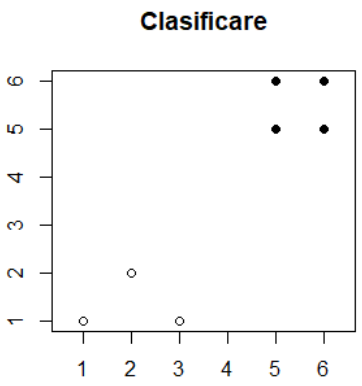
\includegraphics{screenshot001}
	\end{center}
	
	\noindent la clusterizare va arăta astfel:
	\begin{center}
		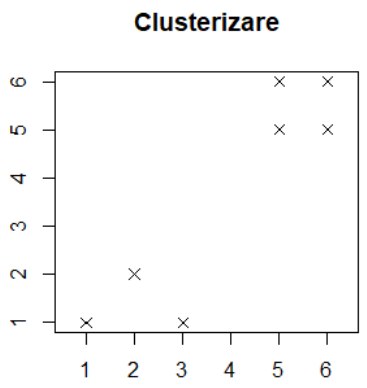
\includegraphics{screenshot002}
	\end{center}
	
	Diferența este că nu mai avem instanțe etichetate (pentru că de acum am zis că facem învățare \textbf{ne}supervizată). Totuși ce putem face cu aceste date? Dacă vă uitați atent la ultimul desen, deși nu avem etichete, observăm că instanțele s-ar grupa în două grupuri (sau clustere): unul în stânga jos și unul în dreapta sus. De fapt, asta vom face: vom încerca să grupăm datele (= să le clusterizăm). 
	
	[După ce le-am grupat, dacă vrem, celor din stânga jos le putem pune o etichetă, iar celor din dreapta sus, o altă etichetă. Astfel, am etichetat setul de date și de acum putem rula, dacă vrem, algoritmi de clasificare.] 
	
	Dar hai să vedem cum se poate face clusterizarea asta...

	\section{Remember}
	\begin{enumerate}
		\item \textbf{produsul scalar}: $$\begin{bmatrix}
		x_1\\
		\vdots\\
		x_n
		\end{bmatrix} \cdot \begin{bmatrix}
		y_1\\
		\vdots\\
		y_n
		\end{bmatrix} = x_1 y_1 + \dots + x_n y_n$$
		Exemplu:
		$$\begin{bmatrix}
		1\\
		2
		\end{bmatrix} \cdot \begin{bmatrix}
		3\\
		4
		\end{bmatrix} = 1\cdot 3 + 2 \cdot 4 = 11$$
		\item \textbf{norma} $p$, $p \geq 1 $: $$\left\Vert \begin{bmatrix}
		x_1\\
		\vdots\\
		x_n
		\end{bmatrix} \right\Vert_p = (|x_1|^p + \dots + |x_n|^p)^\frac{1}{p}$$
		Exemple:
		
		$p=1$
		
		$$\left\Vert \begin{bmatrix}
		1\\
		-2
		\end{bmatrix}\right\Vert_1 = |1| + |-2| = 3$$
		
		$p = 2$
		
		$$\left\Vert \begin{bmatrix}
		1\\
		-2
		\end{bmatrix} \right\Vert_2 = \left\Vert \begin{bmatrix}
		1\\
		-2
		\end{bmatrix} \right\Vert = \sqrt{1^2 + (-2)^2} = \sqrt{5}\text{ - norma euclidiană}$$
		
		\textbf{Implicit}, dacă nu se specifică o altă normă, semnul $\Vert ... \Vert$ se va referi la norma \textbf{euclidiană}.
		
		$p=\infty$
		
		$$\left\Vert \begin{bmatrix}
		1\\
		-2
		\end{bmatrix} \right\Vert_\infty = \max \{|1|,|-2|\} = 2$$
		
		\item distanța $p$ indusă de norma $p$ (vezi \textit{Notițe Seminar 8})
		$$d_p(x,y) = \Vert x - y \Vert_p$$

		\item $\Vert x \Vert_2^2 = x \cdot x$ (o puteți verifica imediat)
		\item $x^2 \stackrel{\text{not.}}{=} x \cdot x$
		\item \textbf{unghiul} dintre 2 vectori
		$$\cos(x,y) = \frac{x \cdot y}{\Vert x\Vert \Vert y\Vert}$$
		Exemplu:
		$$\cos \left(\begin{bmatrix}
		1\\
		0
		\end{bmatrix}, \begin{bmatrix}
		1\\
		1
		\end{bmatrix}\right) = \frac{\begin{bmatrix}
			1\\
			0
			\end{bmatrix} \cdot \begin{bmatrix}
			1\\
			1
			\end{bmatrix}}{ \left\Vert \begin{bmatrix}
			1\\
			0
			\end{bmatrix} \right\Vert \left\Vert \begin{bmatrix}
			1\\
			1
			\end{bmatrix} \right\Vert} = \frac{1}{1 \cdot \sqrt{2}} = \frac{1}{\sqrt{2}}$$
		\begin{center}
			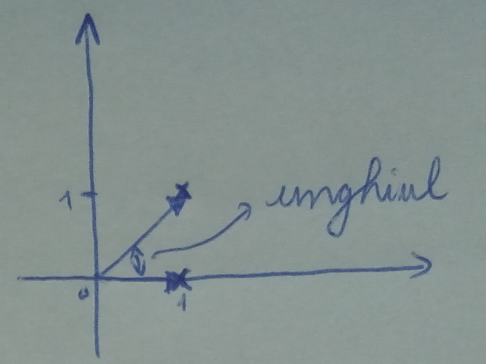
\includegraphics{screenshot003}
		\end{center}
		
	\end{enumerate}

	\section{Clusterizare}
	\begin{itemize}
		\item nu există etichete/coloană output
		\item nu există date de antrenare/de test, ci doar date (deși unii algoritmi pot adaptați pentru a include o nouă instanță într-un cluster...)
		\item coeziune(cluster) $\stackrel{\text{intuitiv}}{=}$ "cât de legate/unite sunt punctele în cluster"
		\item separare(cluster$_1$, cluster$_2$) $\stackrel{\text{intuitiv}}{=}$ "cât de bine distanțate sunt punctele din clusterul$_1$ față de punctele din clusterul$_2$"
		\newpage
		\item poate fi împărțită astfel:
		\begin{enumerate}
			\item \textbf{ierarhică}
			\begin{itemize}
				\item vom forma un arbore care se numește \textbf{dendrogramă}
				\item în funcție de cum construim dendrograma (adică de jos în sus sau de sus în jos), clusterizarea ierarhică se împarte în:
				\begin{enumerate}
					\item clusterizare \textit{\textbf{bottom up}} (sau aglomerativă) - majoritatea exercițiilor vor fi de acest tip
					\item clusterizare \textit{\textbf{top down}} (sau divizivă) - doar ex. 6/pag. 477 este de acest tip
				\end{enumerate}
			\end{itemize}
			\item \textbf{neierarhică}/plată/aplatizată
			\begin{enumerate}
				\item cu asignare \textbf{hard} a instanțelor la cluster, adică având o instanță, spunem că ea aparține unui singur cluster și atât: algoritmul \textbf{k-means}
				\item cu asignare \textbf{soft} a instanțelor la cluster, adică având o instanță, spunem că ea aparține tuturor clusterelor: cu probabilitatea $p_1$ aparține clusterului 1, cu probabilitatea $p_2$ aparține clusterului 2 etc.: algoritmul \textbf{EM/GMM}
			\end{enumerate}
		\end{enumerate}
	\end{itemize}
	
	\section{Clusterizare ierarhică}
	În acest context apare noțiunea de \textbf{similaritate}. Noi vom lucra, de obicei, cu similaritatea dintre doi vectori definită ca \textit{inversul distanței} dintre acei doi vectori. Într-un exercițiu aveți și o similaritate care nu pleacă de la o distanță: este vorba de ex. 32/pag. 539 unde se vorbește despre similaritatea cosinus (care are sens dacă vă gândiți că cos $\in [-1,1]$, cos = 1 dacă unghiul dintre vectori este de zero grade [deci, sunt similare], iar cos = -1 dacă unghiul este de 180 de grade [deci, nu sunt similare]).
	
	Dacă până acum sunteți deja obișnuiți să calculați distanțe între vectori (vezi \textit{Notițe Seminar 8}), în contextul clusterizării ierarhice trebuie să știm să calculăm \textbf{distanțe între clustere} având setată o anumită distanță între vectori. Astfel, setând o distanță $d$ (nu neapărat cea euclidiană) între vectori, vom putea calcula distanța între vectori în mai multe moduri:
	\begin{enumerate}
		\item \textbf{single-linkage}: $d_{sl}(C_1,C_2) \stackrel{\text{def.}}{=} \min\{d(x,y) | x\in C_1, y\in C_2\}$
		
		Exemplu vizual având setată distanța euclidiană: 
		\begin{center}
			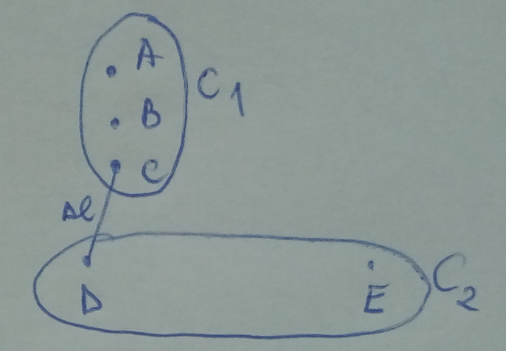
\includegraphics{screenshot004}
		\end{center}
		
		
		$d_{sl}(C_1,C_2) = d(C,D)$
		
		\item \textbf{complete-linkage}: $d_{cl}(C_1,C_2) \stackrel{\text{def.}}{=} \max\{d(x,y) | x\in C_1, y\in C_2\}$
		
		Exemplu vizual având setată distanța euclidiană: \begin{center}
			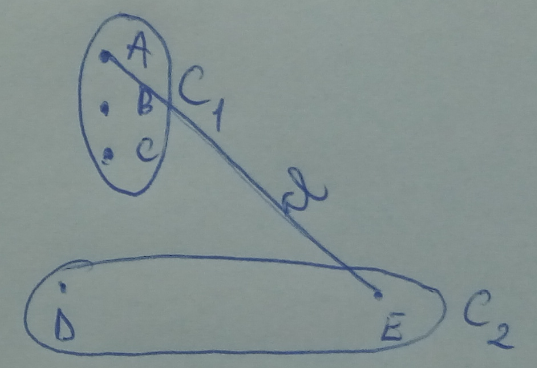
\includegraphics{screenshot005}
		\end{center}
		
		$d_{cl}(C_1,C_2) = d(A,E)$
		
		\item \textbf{average-linkage}: $d_{sl}(C_1,C_2) \stackrel{\text{def.}}{=} avg\{d(x,y) | x\in C_1, y\in C_2\} = \frac{1}{|A| |B|} \sum_{x \in C_1, y\in C_2} d(x,y)$
		
		Exemplu: 
		
		\begin{center}
			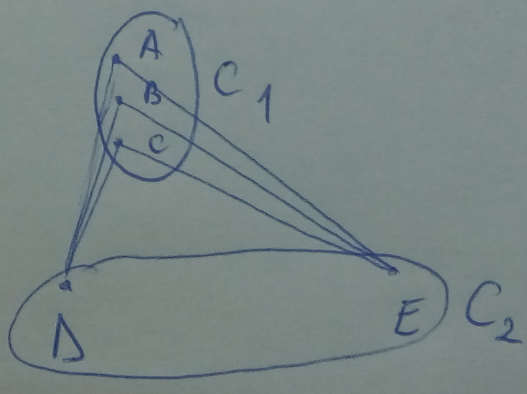
\includegraphics{screenshot006}
		\end{center}
		
		
		$d_{al}(C_1,C_2) = \dfrac{d(A,D) + d(B,D) + d(C,D) + d(A,E) + d(B,E) + d(C,E)}{6}$
		
		\item \textbf{metrica lui Ward}:
		\begin{itemize}
			\item aici vom lucra DOAR cu distanța euclidiană (deci, nu putem seta $d$ să fie altă distanță)
			\item avem nevoie de noțiunea de \textbf{centroid al unui cluster}:
			$$\mu_\text{Cluster} \stackrel{\text{def.}}{=} \frac{\sum_{x \in \text{Cluster}} x}{|\text{Cluster}|}$$
			
			De exemplu: Dacă $\text{Cluster} = \left\{\begin{bmatrix}
			1\\
			2
			\end{bmatrix}, \begin{bmatrix}
			3\\
			4
			\end{bmatrix}, \begin{bmatrix}
			5\\
			6
			\end{bmatrix}\right\}$, atunci
			
			$\mu_\text{Cluster} = \dfrac{\begin{bmatrix}
				1\\
				2
				\end{bmatrix} + \begin{bmatrix}
				3\\
				4
				\end{bmatrix} + \begin{bmatrix}
				5\\
				6
				\end{bmatrix}}{3} = \begin{bmatrix}
			\frac{1+3+5}{3}\\
			\frac{2+4+6}{3}
		\end{bmatrix} = \begin{bmatrix}
		3\\
		4
		\end{bmatrix}$

		Următoarea formulă (pe care o puteți verifica imediat) vă va fi de folos în unele demonstrații: $$\mu_{A \cup B} = \frac{|A| \mu_A + |B| \mu_B}{|A| + |B|}$$
		
		Revenim la metrica lui Ward și o definim:
		
		\begin{align*}
		d_\text{Ward}(C_1,C_2) &\stackrel{\text{def.}}{=} \sum_{x \in C_1 \cup C_2} d^2(x, \mu_{C_1 \cup C_2}) - \sum_{y \in C_1} d^2(y,\mu_{C_1}) - \sum_{z \in C_2} d^2(z,\mu_{C_2})\\
		&\stackrel{\text{dem. ex.30/538-vezi rez.din slide-uri}}{=} \frac{|C_1| |C_2|}{|C_1| + |C_2|} d^2(\mu_{C_1},\mu_{C_2})
		\end{align*}
		
		Exemplu: \begin{center}
			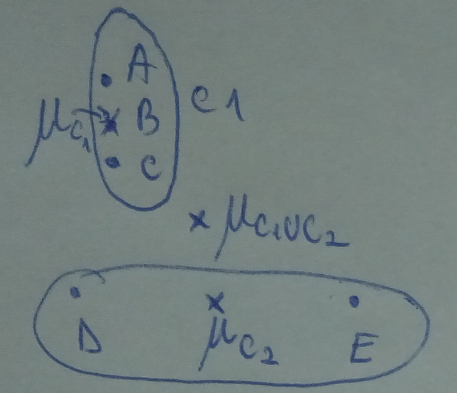
\includegraphics{screenshot007}
		\end{center}
		
		
		\begin{align*}
		d_\text{Ward}(C_1,C_2) &= d^2(A,\mu_{C_1 \cup C_2}) + d^2(B,\mu_{C_1 \cup C_2}) + d^2(C,\mu_{C_1 \cup C_2}) +\\
		&+ d^2(D,\mu_{C_1 \cup C_2}) + d^2(E,\mu_{C_1 \cup C_2}) -\\
		&- (d^2(A,\mu_{C_1}) + d^2(B,\mu_{C_1}) + d^2(C,\mu_{C_1})) -\\
		&- (d^2(D,\mu_{C_2}) + d^2(E,\mu_{C_2}))\\
		& \stackrel{\text{dem.}}{=} \frac{|C_1| |C_2|}{|C_1| + |C_2|} d^2(\mu_{C_1},\mu_{C_2})\\
		&=\frac{3 \cdot 2}{3+2} d^2(\mu_{c_1},\mu_{C_2})\\
		&=\frac{6}{5}d^2(\mu_{C_1},\mu_{C_2})
		\end{align*}
			
		\end{itemize}
		
	\end{enumerate}

	Acum aveți noțiunile de bază ca să aplicați \textbf{algoritmul care formează dendrograma de jos în sus (\textit{bottom up})}. Setăm o distanță între vectori (pentru sl, cl, al) sau nu (pentru Ward). Setăm o distanță între clustere (sl, cl, al sau Ward). În continuare vom lucra cu aceste setări.
	
	Inițial, fiecare punct va fi într-un cluster separat (cluster \textit{singleton}) și va fi o frunză în dendrogramă [deci, inițial avem atâtea clustere câte puncte avem].
	
	La o iterație:
	\begin{itemize}
		\item Calculăm distanțele între oricare două clustere.
		\item Luăm distanța \textbf{minimă} și combinăm clusterele corespunzătoare în dendrogramă trecând astfel de la un nivel inferior în arbore la un nivel superior.
		\item Dacă avem mai mulți candidați pentru distanța minimă, se va specifica o convenție din care să reiasă care clustere vor fi combinate în această iterație.
	\end{itemize} 
	
	Executăm iterațiile până când ajungem la rădăcină (adică ajungem să punem toate punctele într-un singur cluster).
	
	Exemplu: vezi ex. 1a/pag. 468
	
	\textbf{Mențiuni}:
	
	\begin{itemize}
		\item prin tăierea dendrogramei cu o linie orizontală, vom obține o clusterizare \textbf{plată} (vezi desen final din rezolvarea ex. 1b)
		\item având o dendrogramă, putem împărți datele în oricâte clustere dorim (de la 2 la numărul de instanțe); pentru a afla totuși în câte clustere ar fi bine să împărțim datele, ne putem uita la înălțimi; \textbf{înălțimile} în dendrogramă sunt importante!; în exerciții se specifică modul în care se calculează înălțimile; de obicei, ele vor fi invers proporționale cu coeziunea noului cluster SAU direct proporționale cu separarea dintre cele două clustere tocmai unite; din acest motiv vom folosi înălțimile ca să obținem \textbf{numărul natural de clustere}, adică în câte clustere trebuie să împărțim datele (vezi ex. 1b/pag. 468) 
		\item clusterizarea ierarhică asignează \textbf{\textit{hard}} instanțele la clustere
	\end{itemize}

	\newpage
	\textbf{\large{Schemă de final}}
	\begin{enumerate}
		\item Clasificare vs. Clusterizare
		\item Remember
		\item Clusterizare
		\begin{enumerate}
			\item coeziune, separare
			\begin{enumerate}
				\item ierarhică
				\begin{enumerate}
					\item bottom up
					\item top down (vezi ex.6/pag.477)
				\end{enumerate}
				\item neierarhică
				\begin{enumerate}
					\item cu asignare hard a instanțelor la clustere
					\item cu asignare soft a instanțelor la clustere
				\end{enumerate}
			\end{enumerate}
		\end{enumerate}
		\item Clusterizare ierarhică
		\begin{enumerate}
			\item distanță între vectori
			\item similaritate între vectori
			\item distanță între clustere
			\begin{itemize}
				\item single linkage
				\item complete linkage
				\item average linkage
				\item Ward
			\end{itemize}
			\item similaritate între clustere
			\begin{itemize}
				\item cos
			\end{itemize}
			\item dendrogramă, înălțimi în dendrogramă
			\item număr natural de clustere
		\end{enumerate}
	\end{enumerate}
	

	
\end{document}